% Gerado automaticamente. No preambulo do documento use:
% \usepackage{pgfplots}
% \pgfplotsset{compat=1.18}
\definecolor{plotblue}{HTML}{2563EB}
\definecolor{plotorange}{HTML}{D97706}
\definecolor{plotgreen}{HTML}{059669}
\definecolor{plotpurple}{HTML}{7C3AED}
\definecolor{plotgray}{HTML}{374151}
\definecolor{plotred}{HTML}{DC2626}
\definecolor{plotteal}{HTML}{0F766E}
\definecolor{plotslate}{HTML}{64748B}

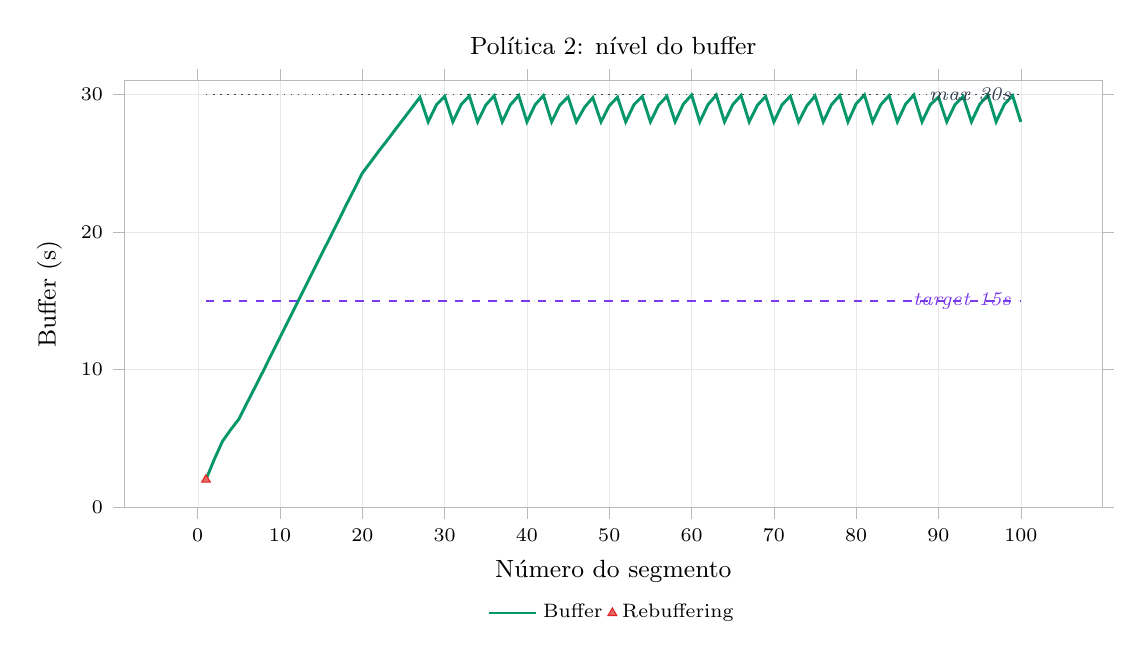
\begin{tikzpicture}
\begin{axis}[
    title={Política 2: nível do buffer},
    xlabel={Número do segmento},
    ylabel={Buffer (s)},
    width=14cm,
    height=7cm,
    grid=major,
    grid style={line width=.12pt, draw=gray!18},
    axis line style={draw=gray!55},
    tick style={draw=gray!55},
    tick align=outside,
    title style={font=\small},
    label style={font=\small},
    tick label style={font=\scriptsize},
    legend cell align={left},
    legend style={at={(0.5,-0.20)}, anchor=north, legend columns=3, draw=none, font=\scriptsize},
    ymin=0,
    ymax=31
]
\addplot+[plotgreen, line width=1.05pt, mark=none] coordinates {
(1,2)
(2,3.46)
(3,4.78)
(4,5.63)
(5,6.4)
(6,7.59)
(7,8.76)
(8,9.94)
(9,11.15)
(10,12.35)
(11,13.55)
(12,14.73)
(13,15.93)
(14,17.13)
(15,18.32)
(16,19.51)
(17,20.69)
(18,21.91)
(19,23.08)
(20,24.28)
(21,25.07)
(22,25.88)
(23,26.64)
(24,27.44)
(25,28.22)
(26,29)
(27,29.79)
(28,28)
(29,29.24)
(30,29.85)
(31,28)
(32,29.25)
(33,29.89)
(34,28)
(35,29.22)
(36,29.89)
(37,28)
(38,29.25)
(39,29.91)
(40,28)
(41,29.25)
(42,29.91)
(43,28)
(44,29.22)
(45,29.81)
(46,28)
(47,29.06)
(48,29.76)
(49,28)
(50,29.17)
(51,29.79)
(52,28)
(53,29.25)
(54,29.84)
(55,28)
(56,29.22)
(57,29.86)
(58,28)
(59,29.29)
(60,29.95)
(61,28)
(62,29.26)
(63,29.95)
(64,28)
(65,29.25)
(66,29.91)
(67,28)
(68,29.21)
(69,29.85)
(70,28)
(71,29.25)
(72,29.87)
(73,28)
(74,29.17)
(75,29.88)
(76,28)
(77,29.25)
(78,29.92)
(79,28)
(80,29.32)
(81,29.96)
(82,28)
(83,29.26)
(84,29.91)
(85,28)
(86,29.29)
(87,29.95)
(88,28)
(89,29.25)
(90,29.8)
(91,28)
(92,29.25)
(93,29.84)
(94,28)
(95,29.27)
(96,29.96)
(97,28)
(98,29.27)
(99,29.91)
(100,28)
};
\addlegendentry{Buffer}
\addplot+[plotpurple, dashed, line width=0.55pt, mark=none, forget plot] coordinates {(1,15) (100,15)};
\node[anchor=east, plotpurple, font=\scriptsize\itshape] at (axis cs:100,15) {target 15s};
\addplot+[plotgray, dotted, line width=0.55pt, mark=none, forget plot] coordinates {(1,30) (100,30)};
\node[anchor=east, plotgray, font=\scriptsize\itshape] at (axis cs:100,30) {max 30s};
\addplot+[only marks, mark=triangle*, mark size=1.8pt, plotred, mark options={solid, fill=plotred!70, draw=plotred}] coordinates {
(1,2)
};
\addlegendentry{Rebuffering}
\end{axis}
\end{tikzpicture}
